\chapter{Foundations and Background}\label{ch:foundations}
%
In this section, we establish the foundational concepts for this dissertation.
We begin by discussing plagiarism and academic integrity. Then, we take an in-depth look at software plagiarism detection, focusing on token-based techniques. We then examine plagiarism generators, which automate code obfuscation, making it more challenging to identify plagiarized origins. Lastly, we introduce model-driven engineering and discuss its significance in the context of modeling education.
%
We intentionally keep these sections concise to ensure practicability\footnote{For more in-depth information, we encourage the interested reader to refer to the referenced literature.}.

\section{On Plagiarism and Academic Integrity}

A wide variety of factors contribute to plagiarism and academic misconduct~\cite{Amigud2019}. To provide some understanding of these factors, the so-called \textit{fraud triangle} by \citet{Cressey1953} can be referenced. While it was originally designed for occupational fraud, it is often used in the context of plagiarism detection~\cite{Albluwi2019}. The fraud triangle identifies three critical aspects for plagiarism to occur:
\begin{enumerate}
    \item \textbf{Motivation:} Students often feel compelled to plagiarize due to high academic pressure, tight deadlines, bad time management, or a lack of confidence in their own abilities and the fear of failure. The intended outcome can be simply passing an assignment or achieving a higher grade.
    \item \textbf{Opportunity:} Students need an opportunity in order to consider plagiarism. This can be, for example, access to peers' solutions. Factors like the lack of routine plagiarism checks further cause this opportunity to grow.
    \item \textbf{Rationalization:} Students may justify their actions with rationalization. While they typically know that their behavior is misconduct, they often try to rationalize it. They may argue that they only copied a small part of that. They are not the only ones to do so.
\end{enumerate}
Note that, in reality, this issue is highly complex and varies for individual cases~\cite{Amigud2019}. However, these three aspects -- motivation, opportunity, and rationalization -- show very well that it is a \textit{human} problem, thus requiring the necessary sensitivity and care. Whatever motivates students to plagiarize, they often delay seeking outside help until they reach the point where they feel they can no longer continue\footnote{From my experience, university students rarely plagiarize purely due to ill intent or disdain for the task at hand; instead, they tend to do so as they consider it the only way out of their situation.}~\cite{Amigud2019}.


\subsection{Plagiarism in Computer Science Education}
Plagiarism in computer science education is more common in certain types of courses and assignments, particularly those that are mandatory for students~\cite{Park2003}. It frequently arises in early-stage courses, especially in large-scale, first-year programming courses~\cite{Yan2018}. Moreover, it is more common for assignments or projects that must be completed individually. Whenever students are allowed to do group work, plagiarism is less frequent.
In addition, plagiarism occurs more frequently when the course or assignment is not necessarily considered essential to a student's primary study area.
%
%One example of a course at Karlsruhe Institute of Technology where plagiarism is more common is the introductory programming courses in which between 750 and 1,000 first-semester students enroll. This combination of factors -- large class sizes, mandatory coursework, and early stages of study -- contributes significantly to the incidence of plagiarism in this course.

Software plagiarism, meaning the plagiarism of source code and other software artifacts like domain models, is challenging to define due to the lack of a universal standard~\cite{Culwin2001}. Definitions of plagiarism vary significantly across institutions and are influenced by course-specific policies, which shape the boundaries of acceptable work~\cite{Simon2013, Simon2014b, Simon2016, novak2023}. Each course must establish its own criteria, often requiring explicit decisions on several factors: whether students may collaborate, the extent to which they can reuse external resources, and which tools they are permitted to use.
With the growing prevalence of generative AI and advanced AI-based auto-complete features in integrated development environments, determining acceptable levels of tool usage has become increasingly complex~\cite{ChatGPTGuide}. Clear guidelines around these factors are essential to maintaining academic integrity, as students may otherwise misunderstand or misinterpret the boundaries of originality and permitted assistance in their coursework~\cite{Simon2016}.

Moreover, in computer science, the definition of plagiarism extends beyond the verbatim copying often associated with text-based assignments~\cite{Cosma2008}. For code and modeling assignments, plagiarism encompasses not only identical or near-identical code but also more subtle forms of reuse.
Thus, plagiarism detection in computer science education faces unique challenges and complexities~\cite{Cosma2008, Murray2010, Simon2016, Simon2013}. 
Students often engage in creative obfuscation strategies such as renaming variables, altering code structure, and inserting redundant statements, which complicates the task of detection~\cite{Novak2019, Karnalim2016}.
The prevalence of digital artifacts and the relative ease of duplicating them facilitates plagiarism~\cite{Kauffman2015}.
Unlike traditional assignments, code and models can be easily manipulated to preserve functionality while concealing the origin.

\subsection{Preventing Plagiarism}

In addition to detecting plagiarism, discouraging plagiarism is a strategy that should be followed as well~\cite{Simon2016, Fincher2019}. Academic institutions should rely on not only reactive policies, where plagiarism is addressed only when discovered but also proactive policies~\cite{Culwin2001}. Note that this includes plagiarism checks.
There are multiple ways how educators can reduce the number of plagiarism cases.

First, educators should communicate what constitutes plagiarism and why it is prohibited~\cite{MirandaRodrguez2024}. It is essential to clarify what specific practices constitute source code plagiarism and what does not, as this is neither trivial~\cite{Simon2014b} nor immediately clear to novice programmers~\cite{Simon2014, Cosma2008}.
Moreover, this should be communicated frequently throughout the course~\cite{Simon2016}.
Setting clear expectations early and reiterating them helps students understand that plagiarism in code includes subtle forms of reuse~\cite{Fincher2019}.
Educators should also clarify guidelines around acceptable resources, including peer code and AI tools, reinforcing the importance of originality~\cite{ChatGPTGuide}.

Another aspect is communicating plagiarism checks. Studies show that communicating that plagiarism checks will be done reduces the number of plagiarism cases~\cite{BerrezuetaGuzman2023, Braumoeller2001}.
This means there should be no secret around using plagiarism detection systems or similar approaches.
Conducting routine plagiarism checks and informing students of these checks can deter dishonesty by emphasizing accountability~\cite{Fincher2019}.

Finally, and maybe most obviously, educators should strive to make the coursework engaging and interesting~\cite{Owens2013}. Assignments that encourage creativity and real-world connections can foster students' sense of ownership over their work. Providing support through office hours, study groups, or forums can further reduce students' temptation to plagiarize~\cite{Perkins2020}.

While discouraging plagiarism is vital, it will not completely prevent plagiarism~\cite{Fincher2019}.
Plagiarism may still occur due to academic pressure, so combining preventive actions with inspection measures is essential~\cite{Culwin2001, Simon2016}. Thus, educators may need to conduct plagiarism checks. For source code plagiarism, plagiarism detection systems can assist with this task.

\subsection{Plagiarism Detection Systems}\label{sec:foundations-pds}
Plagiarism detection systems, often also referred to as plagiarism detectors, enable educators to tackle the problem of plagiarism at scale by helping to seek out plagiarism and deter it in the first place~\cite{Braumoeller2001}. 
A plagiarism detector, despite its name, does not detect plagiarism in a definitive sense, nor does it determine what constitutes plagiarism. Instead, it serves as a tool to highlight potentially suspicious candidates for further investigation based on similarity metrics or other heuristic indicators~\cite{mozgovoy2007}. The final decision regarding whether plagiarism has occurred rests with the educator, who must interpret flagged instances in context~\cite{Prashar20204, Culwin2001}. It is, therefore, essential that plagiarism detection systems are not followed blindly but instead used to guide informed decision-making~\cite{Weber2019, Culwin2001, Saglam2024a}.

Plagiarism detection systems can be generally categorized into two types: \textit{internal}, \textit{local}, or \textit{intra-corpal} detectors compare a set of input artifacts for plagiarism. In contrast, \textit{external} \textit{global}, or \textit{extra-corpal} detectors check an artifact against data snippets from the web and dedicated databases. Internal detectors are more prevalent in computer science education, especially in software plagiarism detection~\cite{Butakov2009, Culwin2001}.
However, both types address the same problem but use different data sources.
This dissertation focuses on \textit{internal} software plagiarism detectors.

\citet{Culwin2001} propose a four-stage process on how to employ plagiarism detection systems in practice:
\begin{enumerate}
    \item \textbf{Collection:} In this initial stage, students submit their work, typically via an online system. The submissions are collected and converted to a standardized format for comparison. The system also tracks which students have submitted, ensuring all expected submissions are collected.
    \item \textbf{Detection:} The collected work is analyzed using a detection system, which compares student submissions against each other for internal plagiarism and against external sources for external plagiarism. The detection system identifies potentially plagiarized pairs by looking for similarities, even in cases of obfuscation.
    \item \textbf{Confirmation:} In this human-led stage, educators review detected similarities manually to determine if they constitute plagiarism. This step is crucial to filter out false positives. Educators confirm true cases of plagiarism by examining whether the similarity is undue and intentional.
    \item \textbf{Investigation:} If plagiarism is confirmed, the case is investigated further to decide on an appropriate response. The student is given an opportunity to explain, and any mitigating circumstances are considered. A penalty may be imposed if plagiarism is conclusively determined following a fair process.
\end{enumerate}
This model provides a structured and rigorous approach to using plagiarism detection systems in education, balancing automated detection with human judgment to ensure fair and accurate results.
This is crucial because, as \citet{Weber2019} puts it, upholding academic integrity is a human responsibility and cannot be left solely to automated approaches.

There are substantial differences between plagiarism detection systems for natural language and source code~\cite{Fincher2019, Simon2013, Simon2014b}.
It is essential to clarify that this thesis does not focus on plagiarism detection for natural languages, as this field employs \textit{entirely} different techniques~\cite{Lancaster2005}, and thus approaches significantly differ from the ones in software plagiarism detection.
%
\citet{Simon2013} discuss four key differences between source code and text in the context of plagiarism detection:
\begin{enumerate}
    \item \textbf{Nature of Originality:} In prose text work, originality is generally tied to the unique expression of ideas and proper referencing. For code, however, reusing and adapting existing code snippets is often an accepted practice, especially in professional environments. Thus, the boundary between inspiration and plagiarism is less evident in code than in text.
    \item \textbf{Detection of Similarities:} Code presents unique challenges for plagiarism detection. Code similarity can be masked through superficial changes, such as altering variable names, spacing, and comments, while maintaining the same logical structure. This makes similarity detection in code more complex and shifts the focus to structure-based detection methods~\cite{Nichols2019}.
    \item \textbf{Referencing Standards:} Code lacks a universal standard for referencing, making it unclear for students how to acknowledge borrowed code properly. In programming, in-line comments or documentation within the code itself may indicate sourced material, but this is less common, unlike a footnote or citation in an essay. Thus, detection systems need means to handle shared code that is not plagiarized.
    \item \textbf{Educational Guidelines:} Universities often provide extensive guidance on avoiding plagiarism in prose but tend to lack equivalent resources for code. This gap in instructional support can lead to confusion among students about what constitutes plagiarism in computing assignments, as students must navigate unspoken norms and rely on personal judgment more frequently than for text-based assessments.
\end{enumerate}

\section{Software Plagiarism Detection}\label{sec:SPD}
A software plagiarism detector analyzes pairs of programs to find similar sections and calculates a similarity score for each pair~\cite{Ottenstein1976}.
Outliers can be analyzed based on these scores, and suspicious pairs are identified and ranked in a list of candidates for human inspection. The resulting information is displayed via histograms, ranked lists, and the results of a clustering analysis~\cite{Novak2021,prechelt2000}.
However, the final decision of identifying plagiarism is left to instructors, given the inherent complexity and ethical considerations involved in this task\footnote{In discussions with other researchers, I usually highlight that plagiarism detectors excel at identifying \textit{structural} similarities in many programs, whereas humans are especially good at recognizing \textit{semantic} similarities between two programs. This is why combining large-scale program analysis and human inspection of suspicious candidates is so effective.}~\cite{Culwin2001, Weber2019}. Plagiarism detectors simply enable the analysis of large datasets and provide evidence for program similarities.

Most approaches for software plagiarism detection compare the structure of the input programs~\cite{Nichols2019, Novak2019}.
They analyze the structure of program elements, such as syntax and control structures, to identify similarities. They do so to capture \textit{intent}, which is the underlying logic and intentional aspects in the program design, which is less likely to be altered significantly when plagiarizing.

Among these \textit{structure-based}~\cite{Nichols2019} approaches, token-based approaches, such as MOSS~\cite{MOSS}, and JPlag~\cite{prechelt2000}, are the most popular tools employed in practice~\cite{Aniceto2021}, with JPlag also being the most references and compared to~\cite{Novak2019} in scientific literature.
%
There is a plethora of other software detection approaches available, and frequently referenced ones include SIM~\cite{SIM}, Sherlock~\cite{Joy1999}, and Plaggie~\cite{Plaggie}.

However, as \citet{Novak2019} notes, most of them are not publicly available, used only by their creators, and mentioned in only one article. Furthermore, they find that many of them are never evaluated against other tools, making their performance questionable\footnote{Some of the approaches who \textit{do} evaluate other tools against others use outdated versions of these tools, thus threatening the validity of their evaluations.}.
%
For a detailed overview of the landscape of software plagiarism detection and a systematic review of obfuscation methods, datasets, and algorithm types, we \textit{strongly} encourage the interested reader to examine the work of \textcite{Novak2019}.

\subsection{Terminology}\label{sec:foundations-terminology}
We describe the terminology for the key concepts of this dissertation in the following. Note that no universal definition of software plagiarism exists~\cite{Culwin2001}, as policies vary between countries, institutions, and courses~\cite{Simon2013, novak2023}. Arguably, the absence of a universal definition is desirable, as it forces institutions to define policies that fit their educational contexts~\cite{Simon2014b, Simon2016}.
Thus, this dissertation \textbf{does not define} what specific actions, structural similarities, or obfuscations between programs constitute plagiarism. Doing so universally is inherently impossible, as this is a decision that educators must make on a case-by-case basis.

Moreover, in computer science, the definition of plagiarism extends beyond the verbatim copying often associated with text-based assignments~\cite{Cosma2008}. For code and modeling assignments, plagiarism encompasses not only identical or near-identical code but also more subtle forms of reuse.
Thus, plagiarism detection in computer science education faces unique challenges and complexities~\cite{Cosma2008, Murray2010, Simon2016, Simon2013}. 
Students often engage in creative obfuscation strategies such as renaming variables, altering code structure, and inserting redundant statements, which complicates the task of detection~\cite{Novak2019, Karnalim2016}.
The prevalence of digital artifacts and the relative ease of duplicating them facilitates plagiarism~\cite{Kauffman2015}.
Unlike traditional assignments, code and models can be easily manipulated to preserve functionality while concealing the origin.

\begin{concept}[Detection Quality] Detection Quality in software plagiarism detection is typically defined by the effectiveness of a system in accurately identifying plagiarism instances among a set of programs.
    Since human inspection is typically the final step in the plagiarism detection process, the term \textit{identifying} involves accurately selecting the correct instances as potential candidates for plagiarism. Importantly, this also means avoiding the misidentification of unrelated programs as plagiarized. Detection quality thus involves balancing sensitivity (the ability to catch as many plagiarism cases as possible) with specificity (the ability to prevent false accusations). Given that most plagiarism detection systems produce results based on calculated similarity scores, we can define detection quality as the extent to which these scores are high for actual plagiarism cases and low for unrelated ones. 
\end{concept}

\begin{concept}[Obfuscation] Obfuscation in software plagiarism refers to any deliberate modification of program code intended to conceal its origin~\cite{Collberg2002}. 
More specifically, it often denotes a code transformation that preserves the semantics but changes the appearance of the original code \cite{zhang2014}.
This is frequently exploited for software plagiarism in educational settings~\cite{Novak2019}.
\end{concept}

\begin{concept}[Obfuscation Attack]
Obfuscation Attacks~\cite{Yuan2018, Hayden2019} aim to avoid detection by strategically altering a plagiarized program, thus obscuring the relation to its original~\cite{Saglam2024b, Saglam2024a}. An obfuscation attack can target automated systems or human inspection. For evading automated detection, such an attack aims to lower the computed similarity value by a detection system for the modified program compared to the original.
To evade human detection, the aim is to alter the appearance of a plagiarized program cosmetically so that its relation to its original is less apparent.
Note the same alterations used for obfuscation attacks can occur when comparing two unrelated programs. Thus, specific types of modifications cannot be used to prove that an obfuscation attack has occurred.
\end{concept}

\begin{concept}[Resilience] Resilience is defined as the ability of a software system to consistently deliver a reliable service despite changes in the system's context or environment. These changes are not necessarily negative; they can just be changes in the frequency and type of interacting entities~\cite{Andersson2021}.
However, considering adversarial scenarios, a system is resilient if it can continue to fulfill its mission despite facing adversity, meaning it maintains its required capabilities even under significant stress that might lead to disruptions. Resilience is crucial because, regardless of how well a system is designed, external factors will eventually challenge its stability~\cite{Firesmith2019}.
\end{concept}
%
\begin{concept}[Obfuscation Resilience] Obfuscation Resilience thus refers to the ability of a detection system to withstand an obfuscation attack~\cite{zhang2014, zhang2014b}.
A resilient detector can accurately identify similarities between original and plagiarized code, even when the plagiarized code has undergone significant obfuscation~\cite{Saglam2022}.
With stronger resilience, the effect of obfuscation attacks becomes negligible. Note that obfuscation resilience does not necessarily include complete immunity, where there is no perceivable effect for an obfuscation attack. Additionally, obfuscation resilience is typically multi-faceted, with a single detector demonstrating varying degrees of resilience against different types of attacks.
\end{concept}

\subsection{Token-based Plagiarism Detection}\label{sec:TPD}

Token-based software plagiarism detection systems rely on the linearization of programs~\cite{Wan2018}.
They combine program tokenization with pairwise comparison to identify matching program fragments~\cite{Lancaster2005}. 
The tokenization step transforms the program's code into a parse tree. A subset of the tree nodes is then extracted as \textit{tokens}, where each stands for a single program element, for example, a control structure, a variable declaration, or a method call~\cite{prechelt2002}.
Unlike graph-based approaches, token-based approaches do not keep a tree-based structure~\cite{liu2006}. Instead, they transform the parse tree in a deterministic manner into an ordered sequence. We refer to this sequence, which represents the structure of a program as \textit{tokens sequence}.

Thus, the tokenization linearizes the parse tree and further abstracts from the underlying code, as not all program elements are tokenized.
According to \citet{prechelt2002}, the extracted token sequence \enquote{\textit{characterizes the essence of a program's structure}}\footnote{This, in my opinion, rather fitting description is somewhat poetic but describes it best.}.
While the structural information concerning control structures, declarations, assignments, and function calls remains intact, specific details such as names, types, values, or comments are excluded.
The token sequences of the programs are then used to find matching subsequences between pairs of programs.

\autoref{fig:code_to_tokens} illustrates the tokenization of program elements for a small example program.
The method \texttt{printSquares} prints the squared values of numbers from 1 to 10 via a simple loop where each iteration calculates and prints the square of the loop variable. On the right, the corresponding tokens represent the structure of the program in a simplified form, abstracting details such as variable names, types, and operators. Program elements of the same type, such as variable declarations, are mapped to tokens of the same type. Note that the indentation of tokens is for readability only.
\autoref{fig:code_to_tokens2} provides another example, this time for a method \texttt{printNumbers}, which prints all consecutive numbers from 0 to a specified maximum in a single line. In this example, we observe that program statements may map to multiple tokens if they contain multiple program elements. However, some program elements, like the empty string literal \texttt{""}, are purposefully omitted during tokenization. Finally, different program elements like parameter declarations and local variable declarations are mapped to the same token type.

\begin{figure}[h]
    \centering
    \begin{minipage}{0.45\textwidth}
        \begin{lstlisting}[label=lst:code,language=Java]
void printSquares() {
    int i = 1;
    while (i <= 10) {
        int square = i * i;
        println(square);
        i++;
    }
}
        \end{lstlisting}
    \end{minipage}
    %\hfill
    \begin{minipage}{0.45\textwidth}
        \begin{lstlisting}[label=lst:tokens,numbers=none]
method start
  variable
  loop start
    variable
    apply
    assignment
  loop end
method end
        \end{lstlisting}
    \end{minipage}
    \caption[Mapping Program Elements to Tokens]{Mapping of program elements (on the left) to their corresponding tokens represented by a textual identifier (on the right). Note that details like names, types, and operators are omitted.}
    \label{fig:code_to_tokens}
\end{figure}

\begin{figure}[h]
    \centering
    \begin{minipage}{0.45\textwidth}
        \begin{lstlisting}[,label=lst:original_code,language=Java]
printNumbers(int max) {
    int[] n = range(0, max);
    String result = "";
    for(int i = 0; i < max; i++) {
        result += n[i];
    }
    println(result);
}
        \end{lstlisting}
    \end{minipage}
    \begin{minipage}{0.45\textwidth}
        \begin{lstlisting}[,label=lst:original_tokens,numbers=none]
method start, variable
  variable, apply
  variable
  loop start, variable, assign
    assign
  loop end
  apply
method end
        \end{lstlisting}
    \end{minipage}
    \caption[Mapping Program Elements to Tokens (Cont.)]{Mapping of program elements (on the left) to their corresponding tokens represented by a textual identifier (on the right). Note that a single statement can map multiple tokens.}
    \label{fig:code_to_tokens2}
\end{figure}

As matching single tokens may lead to false positives, a minimal match length hyperparameter~\cite{prechelt2002} is employed, below which subsequences are no longer considered matches. This hyperparameter is the aforementioned cut-off threshold of the plagiarism detector. It is crucial to control the sensitivity of the matching process.
As the tokens abstract from the code, the comparison is inherently resilient against particular obfuscation attacks, such as renaming, retyping, or obscuring constant values~\cite{prechelt2002}.
This particularly includes immunity against all \textit{lexical}~\cite{Joy1999} attacks.
%However, these detectors are not resilient against insertion-based and reordering-based attacks~\cite{DevoreMcDonald2020}.

To ensure scalability for large datasets, plagiarism detectors employ highly efficient techniques based on hashing and tiling \cite{prechelt2002, MOSS}. As their comparison algorithms, MOSS and Dolos~\cite{Maertens2022} are using winnowing~\cite{Schleimer2003}, while JPlag and Sherlock~\cite{Joy1999} use greedy string tiling with the running Karp-Rabin matching~\cite{Wise1993, Wise1995}.

\subsection{JPlag}\label{sec:found-jplag}
JPlag~\cite{prechelt2000, prechelt2002} is a token-based source code plagiarism detector and was initially developed in 1996 at the Karlsruhe Institute of Technology (then the University of Karlsruhe) in response to the growing need for effective plagiarism detection tools in academic settings, particularly in computer science courses where programming assignments are prevalent.
Over the years, JPlag has undergone several significant updates, including the support of new language and enhancements to its comparison algorithms. Today, JPlag is still actively maintained and developed on\footnote{Disclaimer: the author of this dissertation has been project lead for JPlag since October 2020.}.
%
JPlag is widely used in educational institutions worldwide~\cite{Aniceto2021, Lancaster2004}. In scientific literature, JPlag is the most referenced and compared to tool \cite{Novak2019}.
In the last five years, JPlag has been downloaded over 35,000 times.
JPlag is open-source~\cite{JPlag_GitHub}, freely available, and \ac{GDPR} compliant. Therefore, it is widely used in research on software plagiarism and related topics.
JPlag supports 18 programming languages by providing a dedicated language module for each supported language.

Although JPlag operates like other token-based methods, we will elaborate on its specific process in the following.
A set of programs are given as input. These programs are passed to a corresponding language module, which handles the parsing and tokenization of programs for a given language. A language module either uses a parser API or a (ANTLR) grammar to parse programs. Furthermore, each language module defines which program elements are extracted as tokens and to which specific token type they map.
The tokenized programs are then passed to the comparison algorithm. The tokens of each program serve as the abstraction layer for the program code. Thus, from this point on, the process is language-agnostic, meaning the algorithm is language-independent, and it is irrelevant for comparing programs to which program element a token maps~\cite{prechelt2002}.
The comparison algorithm conducts a subsequence search on pairs of programs. To do that efficiently, it is based on greedy string tiling with the running Karp-Rabin matching~\cite{Wise1993, Wise1995}, which allows the comparison of large sets of programs in very short time frames.
Similarity scores are calculated for each program pair based on the matched subsections.

The similarity scores are stored alongside all relevant programs in a report file, which can then be viewed with a web-based user interface.
In this interface, JPlag provides a list of suspicious candidates, a similarity distribution for all program pairs, clusters of program pairs to detect group plagiarism, and all important metadata.
As the mapping between tokens and program elements is stored, the report viewer can inspect pairs of programs from a side-by-side view, where the matched code is highlighted. This allows educators to inspect suspicious candidates and decide which cases constitute plagiarism.

Due to the aforementioned performance optimizations, JPlag scales well for large datasets.
Specifically, for two programs with \( m \) tokens each, the \textit{worst-case} time complexity for finding a matching is \( O(m^3) \)~\cite{Wise1993, prechelt2000}.
This occurs when the sequences have many short shared subsequences, requiring exhaustive comparisons.
\citet{Wise1993} provides proof for the worst-case runtime complexity.
The \textit{average-case} time complexity is stated to be \( O(m^2) \), which reflects the scenario where there are no significant matches between the sequences~\cite{prechelt2002}. 
Moreover, \citet{Wise1993} makes an informal argument based on experiments stating that a \textit{"more realistic estimate in practice"} is between \(O(m)\) and \(O(m^2)\).
%
It is important to note that this analysis pertains to a \textit{single pairwise comparison}. When comparing \( n \) programs, there are \( \binom{n}{2} \) or \( O(n^2) \) comparisons, leading to an overall \textit{average-case runtime complexity} of \( O(n^2 m^2) \) and overall \textit{worst-case runtime complexity} of \( O(n^2 m^3) \). In practice, this process is often faster due to optimizations, such as token hashing and early termination when matches are found. According to \cite{Wise1993}, it is often observed to be close to linear.

JPlag can be customized via a wide variety of parameters to suit the needs of educators.
It allows users to specify multiple root directories containing input programs for plagiarism checking, enabling educators to analyze programs from various courses, assignments, or years. Directories folders containing programs from previous years can be marked accordingly, preventing them from being checked against each other and using them only to check against newer programs. Users can specify a base program representing a common framework used across all student programs. This feature prevents framework code from being matched and helps to differentiate between original work and code that may be based on a shared template.

JPlag provides options to limit the number of comparisons shown in the results, ensuring that educators can focus on the most significant instances of similarity. Users can also export similarity values to a CSV file for further analysis. The sensitivity of plagiarism detection can be fine-tuned by adjusting the minimum number of tokens required to be considered a match. This feature enables educators to balance between detecting similarities and minimizing false positives.
%
JPlag offers to group similar programs using various clustering algorithms and similarity metrics. Users can choose between different clustering methods, such as agglomerative and spectral algorithms, and different similarity metrics used in the clustering process.

\subsection{Application in Education Practice}\label{sec:survey}
Due to large course sizes, manual plagiarism detection becomes infeasible. Thus, educators rely on software plagiarism detectors. While most students participate in assignments in a fair manner, some have access to the solutions of peers, which they then use as a basis for plagiarism, aiming to minimize the similarity between the plagiarized work and the original while still retaining plausibility to avoid detection~\cite{DevoreMcDonald2020}.

As part of the development effort for JPlag, we conducted an informal survey~\cite{JPlagSurvey2024} among its user base to find out how they use software plagiarism detection in their courses\footnote{Note that this is not a scientific contribution of this thesis, instead just a small-scale survey for development purposes.}. Fifty educators from around the world participated in this survey.
Although the survey participants only represent a fraction of all users, the results can provide valuable insights.

We learned that educators employ JPlag in various computer science courses.
Among the most frequent use cases are introductory programming courses and courses on object-oriented programming.
It is also applied in more advanced courses, including courses on algorithms and data structures, software engineering, functional programming, natural language processing, web development, and scalable systems.
Educators utilize JPlag to check for academic integrity in settings ranging from practical exercises and exams to programming projects and lab work. It is also used across multiple levels of computer science education, from high school to advanced university courses.

The results related to the typical dataset size are illustrated in \autoref{fig:survey-dataset-size}.
Educators typically work with a range of dataset sizes when assessing student programs.
The most common reply was regarding datasets containing between 50 and 200 programs, with 38 percent of replies.
At this size, we expect medium-sized university courses.
The second most common was datasets with less than 50 programs, accounting for 26 percent of replies.
This is the size of smaller university courses and school classes.
Third come datasets between 201 and 500 programs, accounting for 24 percent, denoting the group of large university courses.
Finally, only 9 percent of the educators have datasets of more than 500 programs in their (very large) courses.

The results related to the typical size of programs are illustrated in \autoref{fig:survey-program-size}.
Regarding the size of these programs, three-quarters of respondents reported programs containing between 101 and 1000 lines of code. The most common answer was 101 to 250 lines of code with 40 percent, closely followed by 35 percent for 251 to 1000 lines of code. Only 15\% of respondents reported programs below 100 lines of code, while an even smaller group of 10\% reported programs between above 1000 lines of code.
These results are unsurprising. Programming assignments requiring less than 100 lines of code for a solution are mostly trivial and are thus only needed for the beginning of a learner's path. The groups between 101 and 250 lines of code cover medium-sized assignments that are very common in introductory classes, while the ones between 251 and 1000 lines cover larger assignments and final projects.

The results related to usage frequency are illustrated in \autoref{fig:survey-frequency}.
There are varying usage frequencies for JPlag that are common among educators.
Thirty-two percent of educators use JPlag one or two times per year. This probably involves all educators who conduct a single plagiarism check at the end of the course or semester.
Twenty-two percent of them use JPlag between three and five times yearly, which involves semi-frequent plagiarism checks.
Eighteen percent use JPlag between 6 and 10 times a year, while 22 percent use it more than 10 times per year.
These groups likely contain educators conducting plagiarism checks individually for each assignment or project.
Some replies stated that they never use JPlag. We assume these are responses of educators who just found JPlag or technical personnel who provide JPlag for educators at an institution but do not use it themselves.

The survey results give insights into how and for which settings educators use state-of-the-art software plagiarism detection systems\footnote{My personal teaching experience with an introductory programming course and past discussions with educators confirm these results as well.}.
Thus, we can make assumptions about typical datasets in software plagiarism detection scenarios.

\begin{figure}[p]
\centering
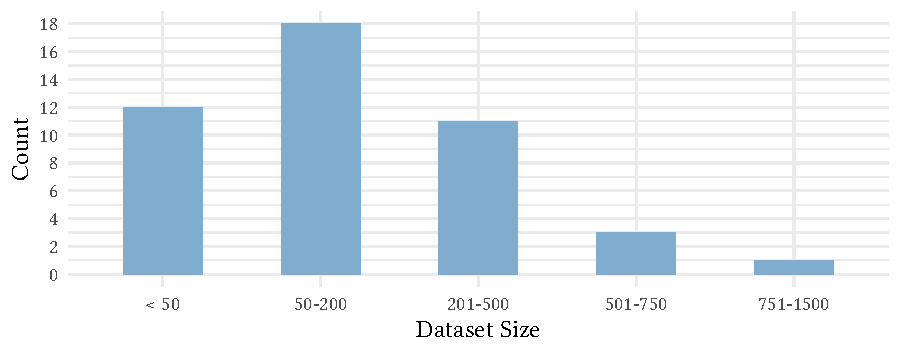
\includegraphics[width=\linewidth]{figures/survey/survey-dataset_size.pdf}
\caption[JPlag Survey: Dataset Size]{Results from the JPlag user survey~\cite{JPlagSurvey2024} regarding the question: \textit{What is your typical dataset size (number of programs)?}.}
\label{fig:survey-dataset-size}
\end{figure}

\begin{figure}[p]
\centering
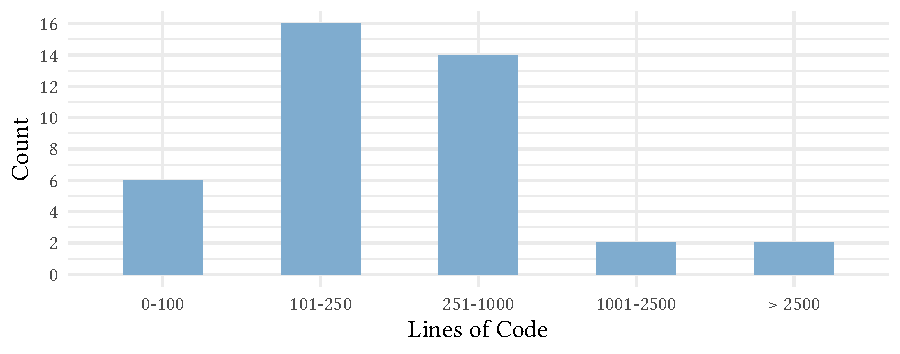
\includegraphics[width=\linewidth]{figures/survey/survey-program_size.pdf}
\caption[JPlag Survey: Program Size]{Results from the JPlag user survey~\cite{JPlagSurvey2024} regarding the question: \textit{What is the estimated average size of a single program (in lines of code)?}.}
\label{fig:survey-program-size}
\end{figure}

\begin{figure}[p]
\centering
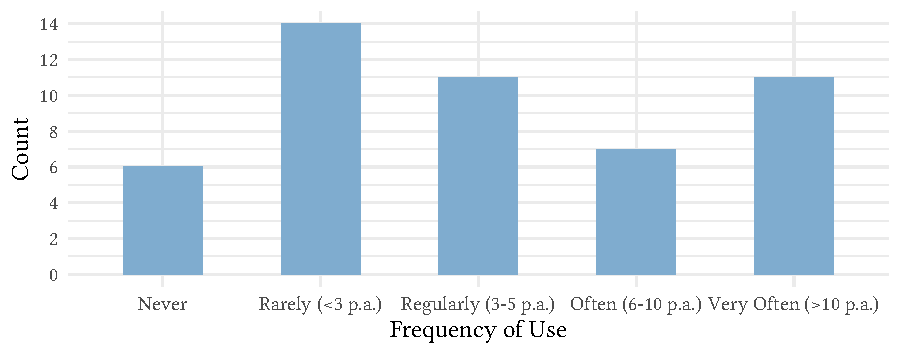
\includegraphics[width=\linewidth]{figures/survey/survey-frequency.pdf}
\caption[JPlag Survey: Usage Frequency]{Results from the JPlag user survey~\cite{JPlagSurvey2024} regarding the question: \textit{How frequently do you use JPlag?}.}
\label{fig:survey-frequency}
\end{figure}

\subsection{Solution Space Problem}\label{sec:SPD-problem}
One of the primary challenges in plagiarism detection lies in the solution space. There are countless correct ways to implement a given solution in programming assignments. 
Thus, unrelated solutions by different students usually do not share many similarities. However, if the complexity of the assignments and hence the degree of freedom in the task is too low or the required solutions are small, the space of possible solutions decreases. Unrelated solutions become increasingly similar, and plagiarism detection becomes more challenging~\cite{Saglam2024b}.

At a certain point, the solution space collapses, strongly limiting the number of distinct solutions. It is no longer possible to differentiate plagiarism instances from accidental similarities between unrelated solutions. Thus, both manual and tool-based plagiarism will not produce any conclusive results and should not be considered.
An example of such an assignment would be writing a piece of code that prints the numbers from one to ten. While there are multiple ways to do it, there are not many. Thus, if students choose a similar or identical way, making assumptions about whether they plagiarize is impossible.

Let us consider a jigsaw puzzle as an analogy. While such a puzzle can be complex, there is only one valid solution. If multiple students now provide the same solutions for such a puzzle, we would not be surprised and would certainly not consider the possibility of plagiarism.
Now, let us consider the task of painting for a given motive; let us say a meadow with a single tree in the center. Here, many possible solutions, maybe even infinite solutions, exist. If now two students produce the same painting with the same colors and brushstrokes, we would be immediately suspicious, as the chance of that happening coincidentally is next to impossible.

This analogy holds true for programming assignments. A complex task requiring a large program to solve it is the counterpart to the painting. Here, plagiarism detection is very effective, and unrelated solutions are dissimilar. However, for trivial programming assignments, for example, used at the beginning of a course for novice programmers, plagiarism detection does not apply. Note that this is an inherent problem and exists both for human inspection and tool-based solutions.  

Educators must be conscious of these limitations. Therefore, plagiarism detectors should be designed to enable teachers to recognize situations where the results lack conclusiveness, enabling them to make well-informed and ethical decisions.

\section{Plagiarism Generators}
Plagiarism generators are programs that implement automated obfuscation attacks in order to generate plagiarism instances for a given input.
In the following, we discuss two algorithmic plagiarism generators~\cite{DevoreMcDonald2020, Broedel2023}. Moreover, we also discuss how generative AI, especially \acp{LLM}, can be exploited to serve as plagiarism generators.

\subsection{\mossad}\label{sec:foundations-mossad}
\textcite{DevoreMcDonald2020} introduce the so-called approach called \mossad\footnote{Capitalization chosen by the author of this dissertation to avoid any possible confusion between terms.}, a software plagiarism generator that rapidly produces obfuscated versions of original programs. Currently, \mossad is limited to C and C++ source code.
\mossad uses techniques inspired by genetic programming to evade plagiarism detection and randomly inserts statements until the similarity to the input computed by a plagiarism detector falls below a user-defined threshold. To keep the inserted statements domain-related and unsuspicious, \mossad uses both existing statements from the input program and a user-defined pool of statements called \textit{entropy}.
\mossad generates multiple variants from a single original, which are not only obfuscated from the original but also among each other due to its indeterministic nature.

During generation, \mossad randomly inserts statements from the pool into the variant.
Next, it checks if the variant still compiles and the semantics are preserved. If either one is not the case, the statement is not used.
After that, it uses a plagiarism detector, such as JPlag or MOSS, to compare the variant to the input program. If the similarity score is below the desired threshold, the corresponding variant is outputted as the final result. If not, this process is repeated.
%
To determine program semantic equivalence, \mossad compares the intermediate representation of programs after compiling both with high-level optimization. %This approach allows it to identify mutations that would be compiled away, such as dead code and redundant assignments.
%
By repeatedly applying mutations randomly, \mossad can create multiple variants that are different enough not to get flagged during plagiarism detection.
Its automatic and efficient nature makes it a potent threat to current plagiarism detection practices.

\mossad demonstrates its effectiveness
against various plagiarism detectors, including MOSS~\cite{MOSS}, Sherlock~\cite{Joy1999}, and JPlag~\cite{prechelt2000,prechelt2002}.
Their approach is mainly designed against token-based plagiarism detectors but has the potential for attacks on other structure-based~\cite{Nichols2019} software plagiarism detectors.

\subsection{PlagGen}
\textit{PlagGen} is a plagiarism generator introduced by \textcite{Broedel2023}.
Originally, it was called \textit{JPlag-Gen}, as it was used to evaluate JPlag. However, we refer to it as PlagGen for the remainder of this dissertation to avoid confusion. PlagGen is inspired by \mossad but has a few key differences. Instead of minimizing the similarity threshold of a target detector, it aims to insert statements at every possible position in the original source code. While it still employs random statements, it is less deterministic than \mossad. However, it avoids issues where some program parts are obfuscated while others are not.

While \mossad exclusively uses insertion~\cite{DevoreMcDonald2020},  PlagGen considers both insertion and reordering of statements.
PlagGen generates plagiarized programs using these two modes separately or in combination.
It first produces a plagiarized program using reordering and then applies insertion on the result, as reordering is considered a weaker attack \cite{Broedel2023}.

PlagGen is primarily designed for Java but could be implemented for other languages.
For insertion, PlagGen uses a similar approach to \mossad by inserting a random statement at a random position and using a compiler to check if the functionality remains unchanged. The key differences include using the Eclipse Compiler for Java (ECJ) instead of the GNU Compiler Collection (GCC), as ECJ can be configured to remove unused variables, thereby supporting most of the functionality of \mossad for Java.
For reordering, PlagGen identifies independent statements that can be swapped without affecting program functionality. It tests for independence based on indentation, control flow keywords, and variable accesses. This approach ensures that only valid modifications are made, thus preserving the program's behavior while effectively obfuscating the code.

While PlagGen is based on the insertion and reordering of statements, this attack can also be modified to employ other types of changes, for example, the automated application of refactoring transformations~\cite{Maisch2024}.


\subsection{Generative Artificial Intelligence}

The rapid development of generative AI, mainly via \acp{LLM}, has introduced new challenges in detecting and preventing plagiarism. AI-based attacks~\cite{Biderman2022}, which leverage these language models, present a growing concern for academic integrity in computer science education. Generative AI can now effectively function as a tool for plagiarism generation~\cite{Khalil_Er_2023}, with \acp{LLM} able to generate and modify code autonomously~\cite{Camara2023, Daun2023}.

Although \acp{LLM} have been critically described as \textit{Stochastic Parrots}~\cite{Bender2021}, they are criticized for lacking proper language understanding (although some researcher argues otherwise~\cite{Hinton2024}) and instead solely rely on statistical patterns.
However, this stochastic imitation is often sufficient to produce human-like code and text for plagiarism. While code generated by generative AI frequently contains flaws~\cite{Choudhuri2024, Camara2023, Ouyang2023}, these imperfections may work in favor of an adversary, as novice students' programs are rarely flawless, making AI-generated code appear realistic in educational settings.
\citet{Biderman2022} demonstrate that pre-trained language models can manipulate code to evade detection by MOSS~\cite{MOSS}, revealing vulnerabilities in current detection methods and emphasizing the need for more robust approaches

Compared to traditional plagiarism generators, generative AI is widely accessible to students. Tools like ChatGPT~\cite{ChatGPT} offer a simple, conversational interface, democratizing access to generative AI and accelerating its adoption~\cite{Saglam2024a}. This \textit{commodification} of generative AI has significantly lowered the barrier for automated obfuscation, making it easier than ever for students to mask plagiarized code, further exacerbating the challenge for educators and detection systems~\cite{ChatGPTGuide}.

For cheating in programming assignments, generative AI can serve two primary purposes in facilitating plagiarism: generating code from scratch and obfuscating existing solutions~\cite{Saglam2024a, Saglam2024b}.
%
The first scenario, \textit{full solution generation}, uses \acp{LLM} to create a solution from scratch based on an assignment description as a prompt. Here, there is an ongoing debate on whether this form of cheating qualifies as plagiarism~\cite{Novak2019, Saglam2024a}.
%
The second scenario, \textit{automatic obfuscation}, involves using generative AI to alter an existing solution's structure without altering its functionality, effectively concealing its origin. This closely resembles human obfuscation practices~\cite{Novak2019}.

Although generated solutions may exhibit higher similarity due to \acp{LLM} semi-deterministic nature, detecting them with low false positives is challenging.
However, current research suggests that automatic obfuscation may be the more effective approach for medium to large assignments, as \acp{LLM} struggle to generate reliable solutions for complex tasks~\cite{Choudhuri2024, Saglam2024b}.
Nevertheless, entirely generated solutions are increasingly feasible for smaller programs, although the effectiveness of these approaches continues to be a topic of research~\cite{Qadir2023}.

\section{Model-Driven Engineering}

Modeling is essential in software development and other fields~\cite{Stahl2006}. It allows designers and engineers to explore design options efficiently, offering stakeholders clear representations of the system being studied. Models enable all participants to understand, analyze, and design complex software and other systems~\cite{Kienzle2024}.

According to the definition by \citet{Stachowiak1973}, a model possesses three fundamental properties: First, it serves as a \textit{mapping} of the archetype it represents. Second, it functions as an abstraction or \textit{reduction} of this archetype, which means not every detail is described. Third, it embodies \textit{pragmatism}, as it is created for a specific purpose.

Model-driven engineering is an approach based on software engineering that considers models as first-class citizens of the development process~\cite{Brambilla2017}. This means that in \ac{MDE}, domain models are primary artifacts alongside code~\cite{Kent2002}.
\cite{Martinez2020} characterizes models as structured data defined by the metamodels they conform to, consisting of model elements that contain attributes and references. These basic building blocks allow for the construction of additional models. 

Metamodels thus describe a set of models, and each model is an instance of its metamodel. Therefore, metamodels exist one \textit{metalevel} above the models they describe~\cite{Stahl2006}.
According to \cite{Bezevin2005}, all \ac{MDE} artifacts, such as model transformations and model queries, can be represented as models themselves, allowing for a uniform treatment of these elements.

The structure of a model typically describes the specifics of the relationships between its elements. In this context, \textit{containment relations}, as recognized in \ac{UML}, indicate stronger relationships that express ownership among model elements.
While models and metamodels are often represented as tree-based structures formed by model elements and their relationships, it is essential to note that this is not universally the case.

To further distinguish between program code and modeling artifacts, it is useful to consider that code typically adheres to executable instructions intended for machine interpretation, while modeling artifacts, which are often domain models, serve as higher-level abstractions aimed at expressing logic or domain-specific structures. While there are executable models~\cite{Seidewitz2014, Fuksa2024}, not all models have well-defined dynamic semantics~\cite{Stahl2006}.

\subsection{Modeling Education}
Modeling is taught in software engineering courses, as modeling languages like \ac{UML} are widely used in practice~\cite{Engels2006, Stahl2006}.
Furthermore, modeling becomes more common in computer science education with the increasing adoption~\cite{Brambilla2017, Hutchinson2011} of model-driven techniques.
Consequently, computer science assignments and exams often include modeling assignments~\cite{Ciccozzi2018, Stahl2006, Saglam2023}, for example, \ac{UML} assignments regarding class, use case, sequence, and activity models.
%
Modeling education includes two aspects~\cite{Kienzle2024}: First, using modeling concepts, languages, and tools. This is more in line with modeling in fundamental software engineering courses. Second, modeling language engineering, metamodeling, and other model-driven concepts.

According to \cite{Ciccozzi2018}, most \ac{MDE} courses are offered at the master's level, leveraging students' prior knowledge in software engineering and modeling. However, some courses are also provided for bachelor's and PhD students. Typically, these courses combine lectures with labs to balance theory and hands-on practice, with many classes having over 90 students.
%
Typical \ac{MDE} courses mainly fall into two categories: domain-specific \ac{MDE} applications using established tools and courses that teach how to develop domain-specific \ac{MDE} tools. These courses cover core concepts and techniques in \ac{MDE}, including language engineering and model transformation. Lectures often focus on meta-modeling to define abstract and concrete syntax and model transformation for code generation. Lab activities allow students to practice with common \ac{MDE} tools like the \ac{EMF}.

While most academic and industrial \ac{MDE} tools are not ideal for teaching modeling~\cite{Kienzle2024}, many education-specific tools exist. In the following, we give some examples of tools for \ac{MDE} education.
%
\textit{Umple}~\cite{Lethbridge21} is an open-source modeling tool that combines graphical and textual interfaces to help students design class diagrams, state machines, and feature models.
\textit{TouchCORE}~\cite{ali2022} is an academic modeling tool centered on reusing and customizing domain-specific languages to enhance students' understanding of complex modeling tasks.
The \textit{Epsilon Playground}~\cite{KolovosGarciaDominguez22} provides web-based examples that allow students to practice with modeling languages directly in the browser, removing the need for complex installations.
The \textit{MDENet} education platform~\cite{Barnett2023} offers a customizable environment where different \ac{MDE} tools can be integrated, allowing educators to create and share interactive modeling activities directly accessible to students online.
\textit{AToMPM}~\cite{Syriani2013b} is a web-based graphical modeling environment that lets students define domain-specific modeling languages with a fully customizable editor.
The \textit{ENCORE} platform~\cite{ENCORE-MODELS23} supports educators in designing personalized learning paths in \ac{MDE} by integrating open educational resources.

\subsection{Modeling Plagiarism Detection}

Modeling assignments are prone to plagiarism due to their complexity and their requirement of domain understanding and problem-solving skills~\cite{Martinez2020}.
However, there is little research on modeling plagiarism and its detection \cite{Martinez2020, Saglam2022, Saglam2023}.
While automated plagiarism detection was proposed decades ago \cite{Ottenstein1976, prechelt2000}, most state-of-the-art plagiarism detectors can only be used with code~\cite{Novak2020}.

While model differencing~\cite{Stephan2013, Kolovos2009} and model clone detection~\cite{Stoerrle2015, Babur2019, Shobha2021} are well researched, these techniques alone are insufficient for plagiarism detection, as they are not resilient against obfuscation attempts~\cite{Wittler2023, Saglam2022, Martinez2020}.
This is unsurprising, as both techniques are not intended for an attacker-defender scenario, e.g., where an attacker purposefully attempts to obfuscate modeling clones or prevent model differencing from correctly deriving the differences between models.

To the author's knowledge, there is only one other approach for modeling plagiarism detection.
\citet{Martinez2020} utilize \emph{Locality Sensitive Hashing} (LSH), an approximate nearest neighbor search mechanism, to detect plagiarism. They embed models into a similarity metric space by transforming them into context-aware fragments that are turned into integer vectors using \textit{minhash} on the names of the fragment's classes, attributes, and operations.
Context-aware fragments are essentially smaller components of the model, which are analyzed in their context, meaning the relationships and properties are considered.
The model signatures are then computed based on these vectors using LSH, and the similarity of any two models is determined by the hamming distance between the two signatures~\cite{Martinez2022}. 

As this approach relies on LSH, it involves several hyperparameters that require adjustment to optimize detection rates for modeling domains. Key parameters include the number of bands, which determines the strictness of signature matching by providing independent opportunities for items to match, and the number of rows per band, which balances precision and recall by adjusting the required signature length for similarity. A higher number of bands with fewer rows increases selectivity, while fewer bands with more rows relax the criteria, identifying more candidate pairs. Proper tuning of these parameters is essential for maximizing the approach's effectiveness~\cite{Martinez2020}.

While this approach effectively detects plagiarism, it combines contextual rather than structural information, making it vulnerable to \textit{some} obfuscation attacks.
The LSH signatures are computed based on names, so their approach is prone to renaming-based obfuscation attacks.
Moreover, this approach does not provide typical traceability features that common approaches for source code plagiarism provide.
This means that, given a similarity score between two models, there is no information about which parts of the models were matched and which parts differed.